%
% File    : project_document.tex
% Author  : Mauricio Villarroel
% Created : Sept 6, 2013
% ____________________________________________________________________________
%
% This program is free software; you can redistribute it and/or modify it
% under the terms of the GNU General Public License as published by the
% Free Software Foundation; either version 2 of the License.
%
% This program is distributed in the hope that it will be useful, but
% WITHOUT ANY WARRANTY; without even the implied warranty of
% MERCHANTABILITY or FITNESS FOR A PARTICULAR PURPOSE. See the GNU General
% Public License for more details.
% ____________________________________________________________________________
%
% DESCRIPTION :
%
% Sample main latex file
% ____________________________________________________________________________


\documentclass{mvdocument}

\makeglossaries
\newabbreviation[longplural={heart rates},description={Heart rate}]{hr}{HR}{heart rate}
\newabbreviation[description={Respiratory rate}]{rr}{RR}{respiratory rate}
\newabbreviation[sort=SaO2,description={Arterial oxygen saturation}]{sao2}{\ensuremath{SaO_2}}{arterial oxygen saturation}
\newabbreviation[sort=SpO2, description={Peripheral oxygen saturation, as measured by a pulse oximeter}]{spo2}{\ensuremath{SpO_2}}{peripheral oxygen saturation}


%
% Project author and metadata
%

\title     {Your title}
\author    {Author's name}
\college   {Your college name}
\university{University of Oxford}
\universitylogo{oxford-logo}       % File name of the logo
\supervisor{Supervisor's name}
\degreedate{Hilary Term, 2048}

%
% Document contents
%

\begin{document}

\frontmatter

\maketitle

\begin{declaration}

I declare that this thesis is entirely my own work and, except where stated, describes my own research.

\bigbreak
\bigbreak

\noindent The author

\noindent XXX College

\end{declaration}

\begin{dedication}
 
 \epigraph{ 
 \textit{\large{Dedicated to very important people} } }
 {}

\end{dedication}

\begin{acknowledgements}

\lipsum[2-4]

\null\vfill
\noindent This thesis was created using the \LaTeX\ typesetting system.

\end{acknowledgements}

\begin{abstract}
    
\lipsum[2-4]

\end{abstract}


\tableofcontents
\listoffigures
\listoftables
\listofabbreviations

\mainmatter

%\layout  %Used temporarly for checking layout

\chapter{Introduction}
\label{chapter:introduction}

It is widely reported, notably by the World Health Organisation \cite{stroetmann2010can}, that global changes in population demographics, the increased incidence of chronic diseases and the unmet needs for more personalised care are trends that need new integrated approaches to health and social care. 

\lipsum[2-4]

\section{Monitoring of vital signs}

The standard vital signs include temperature, \af{hr}, \af{rr}, blood pressure and, when appropriate, \af{spo2}. The routine measurement and interpretation of these vital signs is a core component of the physiological assessment of most patients \cite{prior1977physical,goldberg2005practical}, as they can provide critical information about the underlying state of their health. 

\lipsum[2-4]

\section{Clinical need}

\lipsum[2-4]

\section{Objectives}

\lipsum[2-4]

\section{Contributions}

\lipsum[2-4]

\section{Outline of document}

\Cref{chapter:literature_review} discusses .... . The clinical study undertaken as part of this project is presented in \Cref{chapter:dataset} with a detailed description of the patient population, the data collection process and an overview of the main vital signs used as the reference data....

\lipsum[2-4]

\chapter{Literature review}
\label{chapter:literature_review} 


\section{Introduction}

\lipsum[2-4]

\section{Review of previous methods}

\lipsum[2-4]

\section{Conclusion}

\lipsum[2-4]

\chapter{Dataset}
\label{chapter:dataset} 


\section{Introduction}

\lipsum[2-4]

\section{Clinical study design}

\lipsum[2-4]

\section{Instrumentation}

\lipsum[2-4]

\begin{figure}[tbh]
  \centering
  \subbottom[]{
    \label{fig:grasshopper:lens}
    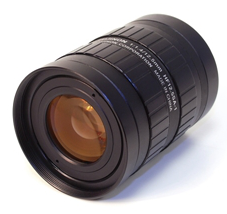
\includegraphics[width=0.2\linewidth,keepaspectratio=true]{fujinon-hf125sa_lens}
  } 
  \subbottom[]{
    \label{fig:grasshopper:camera}
    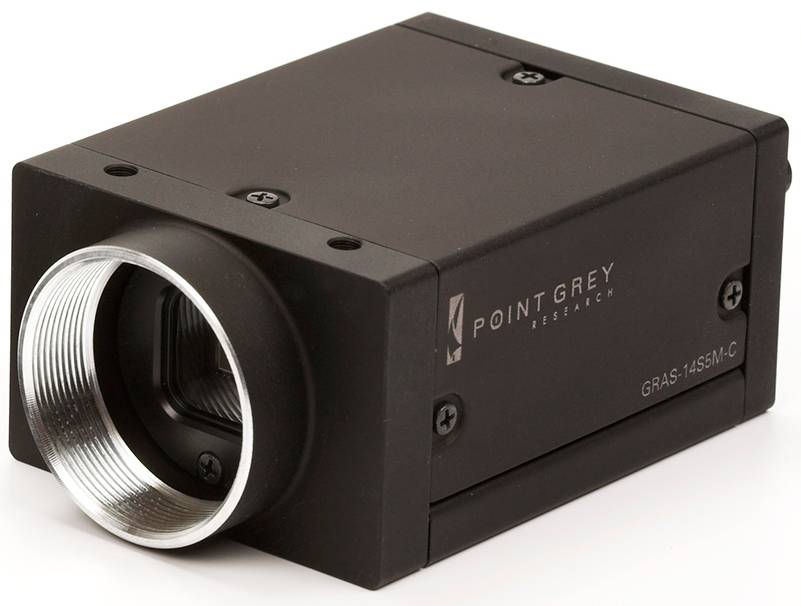
\includegraphics[width=0.22\linewidth,keepaspectratio=true]{grasshopper2}
  }
  \subbottom[]{
    \label{fig:grasshopper:sensor}
    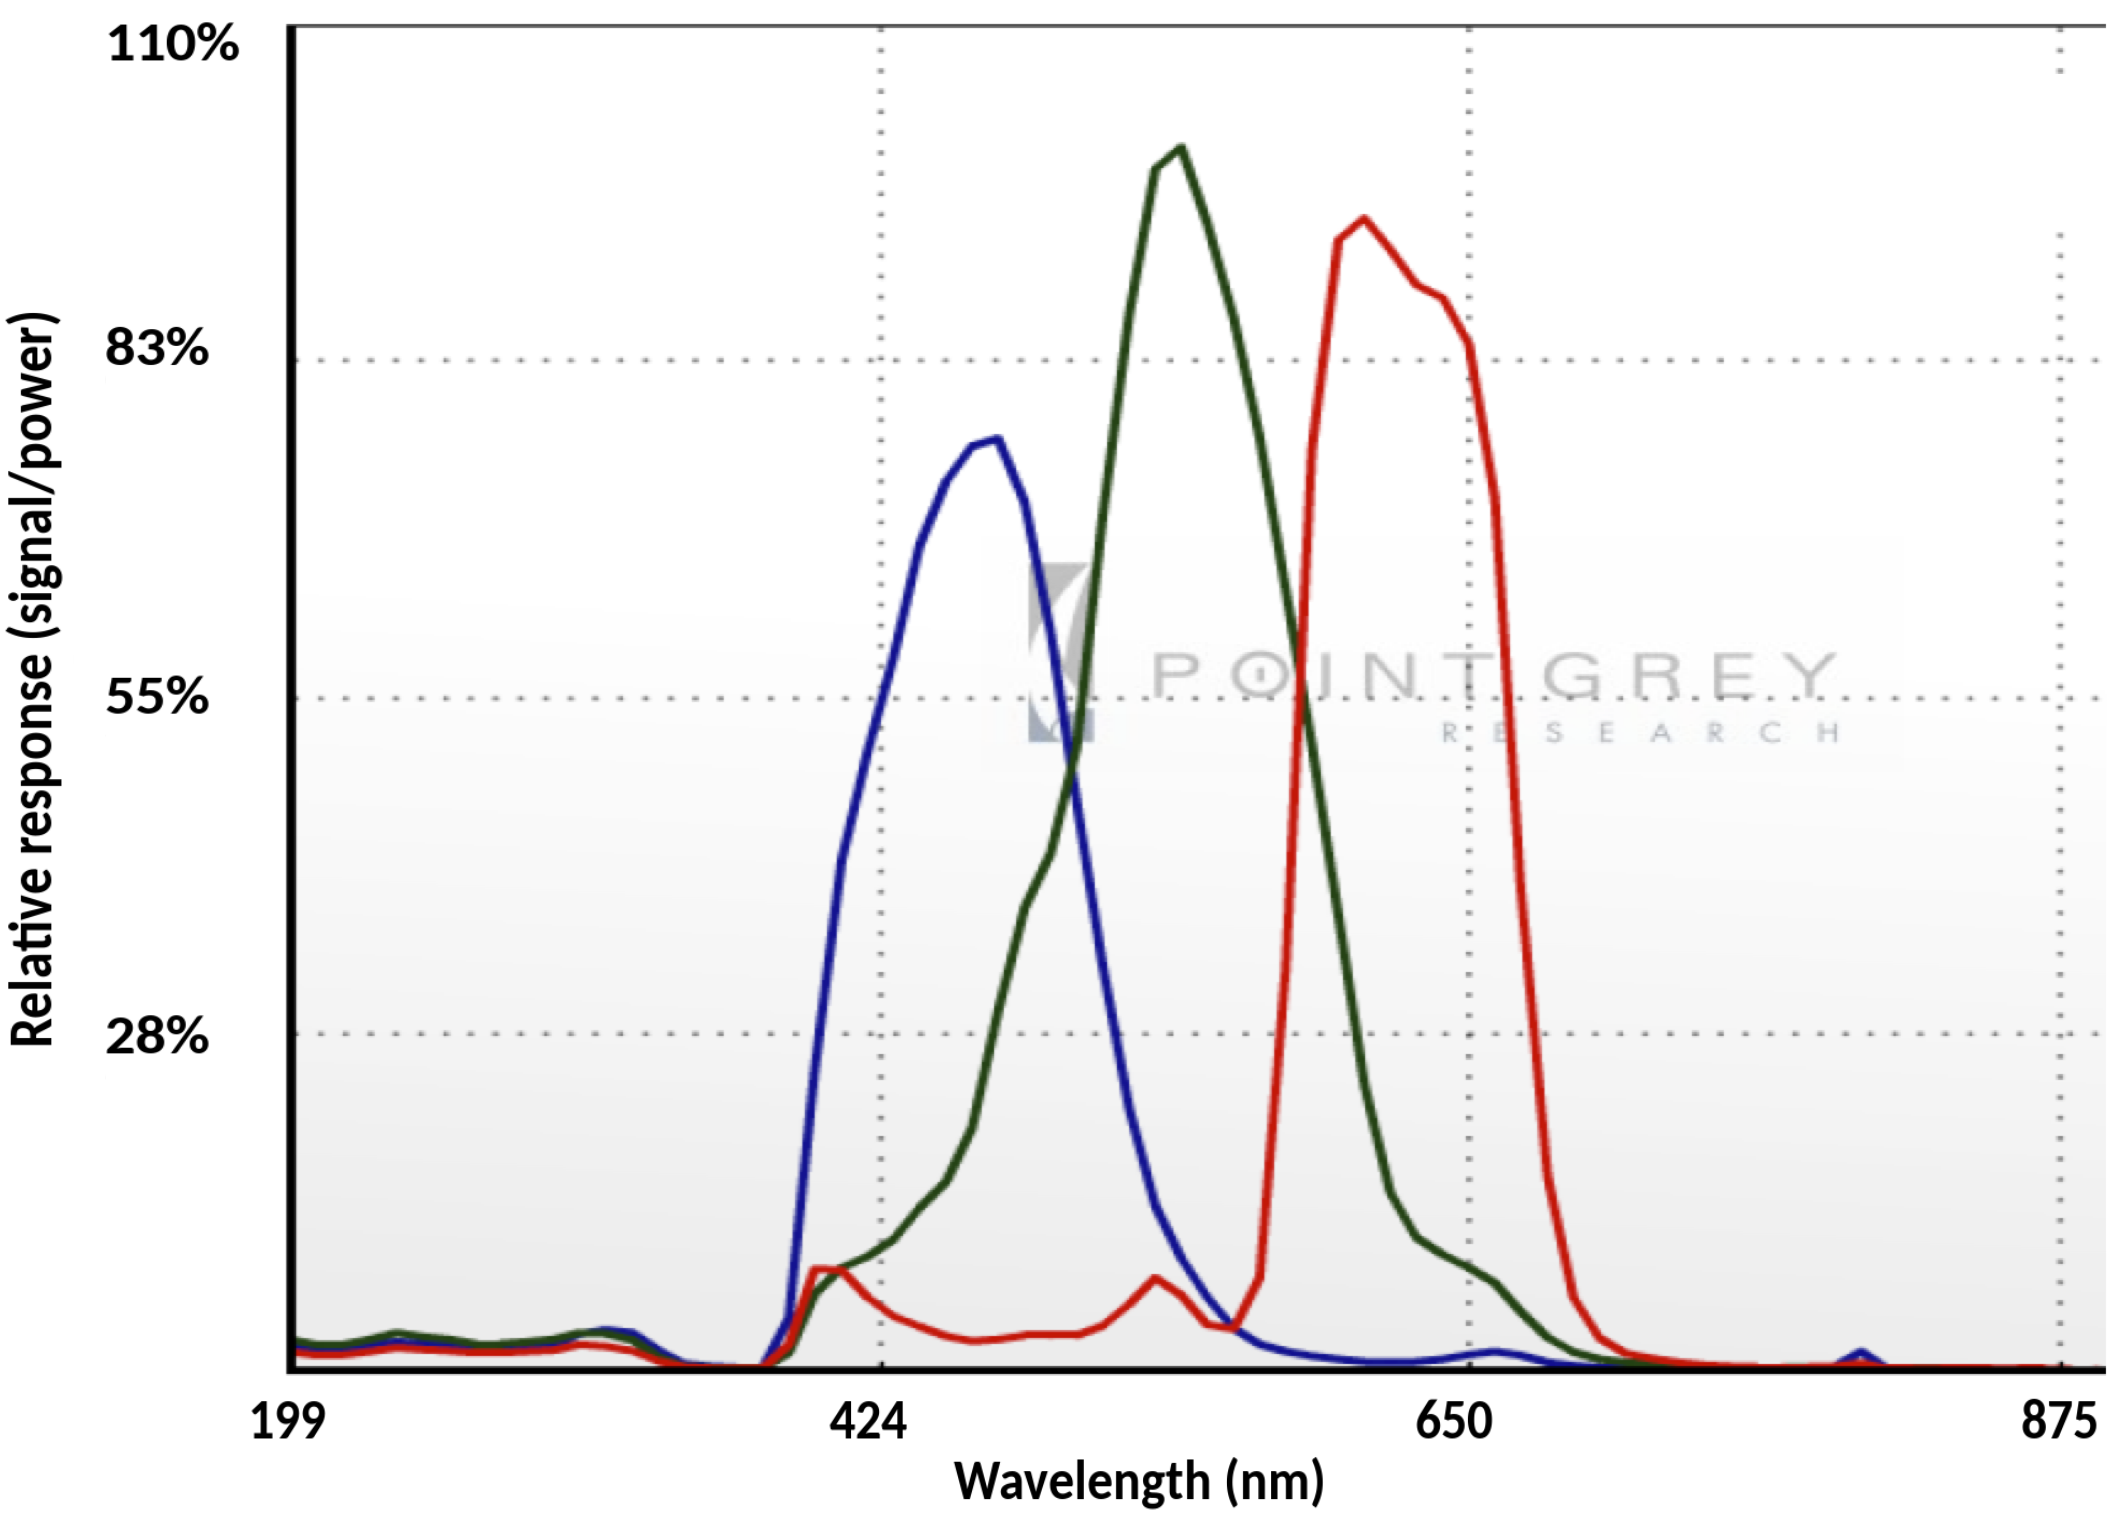
\includegraphics[width=0.45\linewidth,keepaspectratio=true]{grasshopper2_sensor}
  }
  \caption[The PointGrey Grasshopper2 video camera]
  {
  The video camera used in the study:
  \subcaptionref{fig:grasshopper:lens}   Fujinon HF12.5SA-1 lens,
  \subcaptionref{fig:grasshopper:camera} PointGrey Grasshopper2 camera module.
  \subcaptionref{fig:grasshopper:sensor} Response curve for the red, green and blue wavelengths from the image sensor inside the Grasshopper2 camera: Sony ICX625 2/3" progressive scan CCD (Source: PointGrey).
  }
  \label{fig:grasshopper}
\end{figure}

\Cref{fig:grasshopper} shows the video camera used in the study ...

\lipsum[2-4]

\Cref{table:grasshopper2_specs} describes the ...

\begin{table}[bth]
  \centering
  \caption[General features and specification for the PointGrey Grasshopper2 camera]
  {
  General features and specification for the PointGrey Grasshopper2 camera. (Source: PointGrey)}
  {\small
   \singleTableRowHeight
   \begin{tabular}{ll}
     \tableHeaderStart
        \tableHCell{Item} & \tableHCell{Description} \\
     \tableHeaderEnd
     Imaging Sensor        & Sony ICX625 2/3" progressive scan CCD \\
     Image size (pixels)   & 2448 (H) x 2048 (V)                   \\
     Pixel Size            & 3.45 \si{\micro\metre} x 3.45 \si{\micro\metre} \\
     A/D Converter         & AD9977 14-bit, dual-channel           \\
     Max frame rate        & 15 FPS                                \\
     Video Data Output     & 8, 12, 16 and 24-bit digital data     \\
     Gain \& Exposure                  & Automatic/Manual/One-Push              \\
     Lens Mount            & C-mount                                \\
     Interface             & Gigabit Ethernet                       \\
     Physical dimensions   & 44 (W) mm x 29 (H) mm x 58 (L) mm \\
     \hline 
   \end{tabular}
  }
  \label{table:grasshopper2_specs}
\end{table}

\lipsum[2-4]

\section{Patient population}

\lipsum[2-4]

\subsection{Demographics}

\lipsum[2-4]

\subsection{Vital signs}

\lipsum[2-4]

\section{Conclusion}

\lipsum[2-4]
\chapter{Proposed method 1}
\label{chapter:method_1} 


\section{Introduction}

\lipsum[2-4]

\section{Overview of the estimation process}

\lipsum[2-4]

\section{Methods}

\lipsum[2-4]

\section{Results}

\lipsum[2-4]

\section{Discussion}

\lipsum[2-4]

\section{Conclusion}

\lipsum[2-4]
\chapter{Proposed method 2}
\label{chapter:method_2} 


\section{Introduction}

\lipsum[2-4]

\section{Overview of the estimation process}

\lipsum[2-4]

\section{Methods}

\lipsum[2-4]

\section{Results}

\lipsum[2-4]

\section{Discussion}

\lipsum[2-4]

\section{Conclusion}

\lipsum[2-4]
\chapter{Conclusion and future work}
\label{chapter:conclusion} 


\section{Introduction}

\lipsum[2-4]

\section{Clinical study}

\lipsum[2-4]

\section{Propsed method}

\lipsum[2-4]

\section{Future work}

\lipsum[2-4]

\section{Concluding remarks}

\lipsum[2-4]


\appendix

\chapter{Appendix title}
\label{appendix:appendix_1} 


\lipsum[2-4]

To estimate the location of a step change, a Bayesian change point detection algorithm based on \cite{Ruanaidh1996} and \cite{adams2007bayesian} is used in the thesis. Given a data sequence $x$ of $N$ samples with Gaussian noise added:

\begin{equation}
    \centering
      x_i=\begin{cases}
          \mu_1 + \epsilon_i, & \text{if $i<m$}.\\
          \mu_2 + \epsilon_i, & \text{otherwise}.
          \end{cases}
    \label{eq:app:cp:5.1}
\end{equation}

where the noise samples $\epsilon_i$ are assumed to be independent and $m$ is the step change location. The likelihood of the data is given by the joint probability of the noise samples $\epsilon_i$: 

\begin{equation}
    \centering
    P(x|\{\mu_1\mu_2\sigma m\}) = \prod\limits_{i=1}^N P(\epsilon_i)
    \label{eq:app:cp:5.2}
\end{equation}

where $\sigma$ is the standard deviation of the Gaussian noise;  $\mu_1, \mu_2$ and $\sigma m$ are the known time series parameters. The probability density function for the noise samples is defined by:

\begin{equation}
    \centering
    P(\epsilon) = \frac{1}{\sigma \sqrt{2 \pi} }  e ^{ - \frac{ (\epsilon - \mu)^2 } {2\sigma^2} }
    \label{eq:app:cp:noise_pdf}
\end{equation}

\lipsum[2-4]
\chapter{Appendix title}
\label{appendix:appendix_2} 


\lipsum[2-4]


\backmatter 

\listofreferences{references}

\end{document}
